\documentclass{article}

%============================================
%============================================
%===== PACKAGES AND DOCUMENT SETTINGS =====
%============================================
%============================================

%===== General margin setup =====
\setlength{\oddsidemargin}{0.25 in}
\setlength{\evensidemargin}{-0.25 in}
\setlength{\topmargin}{-0.6 in}
\setlength{\textwidth}{6.5 in}
\setlength{\textheight}{8.5 in}
\setlength{\headsep}{0.75 in}
\setlength{\parindent}{0 in}
\setlength{\parskip}{0.1 in}

%===== Packages that I normally like to use
\usepackage{amsmath,amssymb} %General math symbols and stuff
\usepackage[mathscr]{euscript} %To use script letters with \mathscr{}
\usepackage{amsthm} %To be able to write Definitions, Theorems, etc.
\usepackage{graphicx} % To scale equation*s and put figures wherever
\usepackage{framed} % To be able to frame theorems and stuff with begin{framed} ... \end{framed}
\usepackage{float} %To be able to place figures exactly where I want with [H]
\usepackage{multirow}
\usepackage{color}
\usepackage{cite}
\usepackage[hidelinks, breaklinks=true]{hyperref} %To be able to use links inside the document; [hidelinks removes the ugly red boxes]
\usepackage{xcolor}  \definecolor{shadecolor}{rgb}{.95,.95,.95}  %To put a shaded region
%\usepackage[font=footnotesize]{caption}
\usepackage{nicefrac} %to put small fractions nicely with \nicefrac{1}{2}
\usepackage{ragged2e}	%to put \justify
\usepackage[shortlabels]{enumitem}	%To put letters in enumerate with begin{enumitem}[(a)]
\usepackage{amsmath}

%===== Algorithm setup =====
\usepackage[ruled,vlined]{algorithm2e}

%===== Example setup =====
\usepackage{mdframed}
\usepackage{changepage}
\newmdenv[
  topline=false,
  bottomline=false,
  skipabove=\topsep,
  skipbelow=\topsep
]{siderules}

%===== Theorems, lemmas, definitions, etc.
\theoremstyle{definition}
\newtheorem{myDefinition}{Definition}
\newtheorem{myTheorem}{Theorem}
\newtheorem{myLemma}{Lemma}
\newtheorem{myCorollary}{Corollary}
\newtheorem{myProposition}{Proposition}
\newtheorem{myExample}{Example}
\newtheorem{myExercise}{Exercise}
\newtheorem{myRemark}{Remark}
\newtheorem{myConjecture}{Conjecture}

%===== Page counters, theorem counters, etc.
\newcounter{lecnum}
\renewcommand{\thepage}{\thelecnum-\arabic{page}}
\renewcommand{\thesection}{\thelecnum.\arabic{section}}
\renewcommand{\theequation}{\thelecnum.\arabic{equation}}
\renewcommand{\thefigure}{\thelecnum.\arabic{figure}}
\renewcommand{\thetable}{\thelecnum.\arabic{table}}
\renewcommand{\themyDefinition}{\thelecnum.\arabic{myDefinition}}
\renewcommand{\themyTheorem}{\thelecnum.\arabic{myTheorem}}
\renewcommand{\themyLemma}{\thelecnum.\arabic{myLemma}}
\renewcommand{\themyCorollary}{\thelecnum.\arabic{myCorollary}}
\renewcommand{\themyProposition}{\thelecnum.\arabic{myProposition}}
\renewcommand{\themyExample}{\thelecnum.\arabic{myExample}}
\renewcommand{\themyExercise}{\thelecnum.\arabic{myExercise}}
\renewcommand{\themyRemark}{\thelecnum.\arabic{myRemark}}
\renewcommand{\themyConjecture}{\thelecnum.\arabic{myConjecture}}

%===== Header box =====
\newcommand{\lecture}[3]{
\pagestyle{myheadings}
\thispagestyle{plain}
\newpage
\setcounter{lecnum}{#1}
\setcounter{page}{1}
\noindent
\begin{center}
\rule{\textwidth}{1.6pt}\vspace*{-\baselineskip}\vspace*{2pt} % Thick horizontal line
\rule{\textwidth}{0.4pt}\\[1\baselineskip] % Thin horizontal line
\vbox{\vspace{2mm}
\hbox to 6.28in { {\bf CS 4980/6980: Predictive Data Analysis } \hfill $\copyright$ Spring 2018 }
\vspace{4mm}
\hbox to 6.28in { {\Large \hfill Lecture #1: #2  \hfill} }
\vspace{4mm}
\hbox to 6.28in { {\scshape Instructor: Daniel L. Pimentel-Alarc\'on}   \hspace{3mm}\hfill Scribed by: #3 }}
\vspace{-2mm}
\rule{\textwidth}{0.4pt}\vspace*{-\baselineskip}\vspace{3.2pt} % Thin horizontal line
\rule{\textwidth}{1.6pt}\\[\baselineskip] % Thick horizontal line
\end{center}
\markboth{Lecture #1: #2}{Lecture #1: #2}
\vspace*{4mm}
}

%====================================
%====================================
% ===== VARIABLES AND COMMANDS =====
%====================================
%====================================


%===== Some frequent commands that I use =====
\newcommand{\bs}[1]{\boldsymbol{#1}} %bold symbol
\newcommand{\hatt}[1]{\boldsymbol{\hat{#1}}} %bold hat
\newcommand{\careful}{\textcolor{red}}
\newcommand{\comment}{\textcolor{blue}}
\newcommand*\rot{\rotatebox{90}} %To rotate text in table
\newcommand*{\Scale}[2][4]{\scalebox{#1}{\ensuremath{#2}}} % To scale variables in equation*s

%===== In case you want to add colored text =====
\newcommand{\blue}{\textcolor{blue}}

%===== Miscelaneous math symbols =====
\def \R{\mathbb{R}}
\def \Pr{\mathsf{P}}
\def \T{\mathsf{T}}
\def \c{\mathsf{c}}
\def \spn{{\rm span}}
\def \Ord{\mathscr{O}}
\def \<{\langle}
\def \>{\rangle}
\DeclareMathOperator*{\argmin}{arg\,min}
\DeclareMathOperator*{\argmax}{arg\,max}

%===== Common scalars that will be used throughout =====
\def \D{{\hyperref[DDef]{{\rm D}}}} % ambient Dimension
\def \N{{\hyperref[NDef]{{\rm N}}}} %Number of samples
\def \xi{{\hyperref[xiDef]{{\rm x}}}} % a scalar variable x

%===== Common vectors that will be used throughout =====
\def \xx{{\hyperref[xxDef]{\bs{{\rm x}}}}} % a vector x
\def \yy{{\hyperref[yyDef]{\bs{{\rm y}}}}} % a vector y

%===== Common matrices that will be used throughout =====
\def \I{{\hyperref[IDef]{\bs{{\rm I}}}}} % Identity matrix
\def \X{{\hyperref[XDef]{\bs{{\rm X}}}}} % Data matrixm

%Indices that will be used throughout.
\def \i{{\hyperref[iDef]{{\rm i}}}} % index used for samples, usually goes from 1 to N

%=====================================
%=====================================
%===== HERE BEGINS THE DOCUMENT =====
%=====================================
%=====================================

\begin{document}

%===== Lecture's number, title, and students' names.
\lecture{8} % Lecture number
{Nearest Neighbor, k-Nearest Neighbors, and k-Means} % Lecture title
{Harnoor Singh and Jason Vaughn} % Students' names

%===== Section
\section{Introduction}
\textbf{Nearest Neighbor} is a method used for classification of data points through supervised learning. For an instance, given a labeled data set divided it to 2 or more classes, predict which class a new point $\textbf{X}_{n+1}$ will belong to. k-Nearest Neighbors is used as a better alternative to this algorithm.

\textbf{k-Nearest Neighbors}  is a non-parametric method used for classification and regression. As the labels are given to us, this method is called a Supervised Learning Model. \\
Goal: For an instance, given a labeled data-set divided into several classes, predict which category a new \textbf{X} point will lie.\\
This can be used for searching for semantically similar objects or even recommender systems.

\textbf{k-Means Clustering}  is a clustering algorithm that tries to partition a set of points into K sets (clusters) such that the points in each cluster tend to be near each other. It is unsupervised because labels (classes/categories) are not given for the set of points.\\
This is useful for things such as clustering customers and segmenting them or trying to figure out where to open a new branch of a store with delivery.

\section{Nearest Neighbor}

In the Nearest Neighbor algorithm, the goal is to find the classifier of a new data point while being given a set S of points with known classifiers. The classifier of this new data point $X_{n+1}$ is the classifier, $K_{n+1}$, of the nearest point to $X_{n+1}$. This is accomplished by finding the point $i^*$ where:

\begin{equation}
i^* = \argmin_{i\in \{1,...,n\}} ||\textbf{X}_{n+1} - \textbf{X}_i||_2 ^2
\end{equation}

The classifier that is given to $i^*$ is now also given to $X_{n+1}$, meaning:
\begin{equation}
K_{n+1} = K_{i^*}
\end{equation}

\begin{figure}[H]
	\centering
	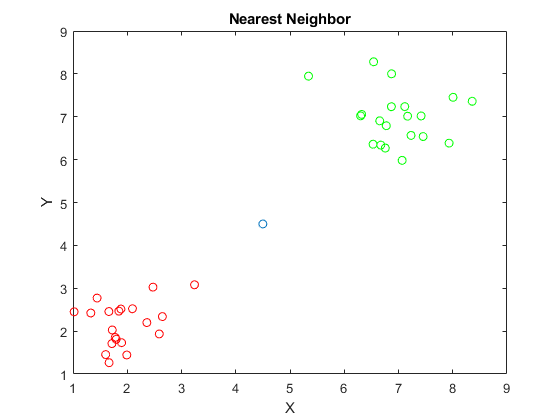
\includegraphics[width=0.5\linewidth, scale=0.5]{Nnbefore.png}
	\caption{We only need to look at the closest neighbor to our new point.}
\end{figure}

\begin{figure}[H]
	\centering
	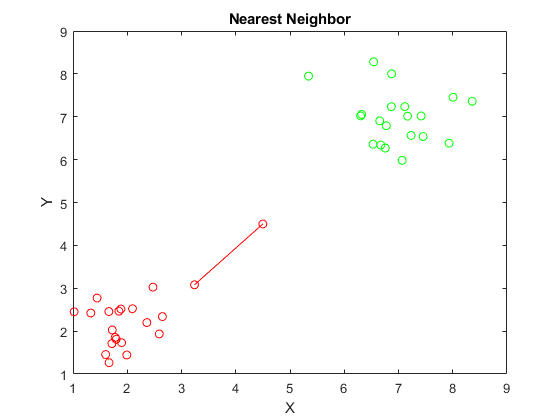
\includegraphics[width=0.5\linewidth, scale=0.5]{Nnafter.png}
	\caption{Looking at the nearest point only, the new point is classified as green.}
\end{figure}

\section{k-Nearest Neighbors}

k-Nearest Neighbors is just an extension of the Nearest Neighbor algorithm. The k in this algorithm is how many neighbors it is to consider. As such, Nearest Neighbor can be considered as 1-Nearest Neighbor. For k-Nearest Neighbors, we first find the k-closest points to a new point, $\textbf{X}_{n+1}$. From this, we take the argmax of the number of each classifier within our neighboring points. If two classifiers are tied for the most, we may randomly choose one of the tied classifiers for determining which our new point belongs to. k is usually chosen empirically.

\begin{figure}[H]
	\centering
	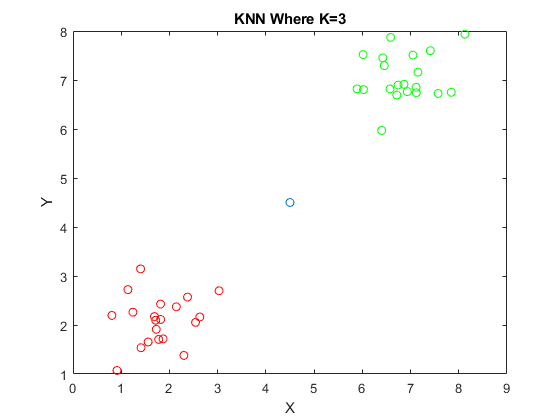
\includegraphics[width=0.5\linewidth, scale=0.5]{Knn3before.png}
	\caption{We need to look at the closest neighbors to find the new black point's classifier. We will use k = 3.}
\end{figure}

\begin{figure}[H]
	\centering
	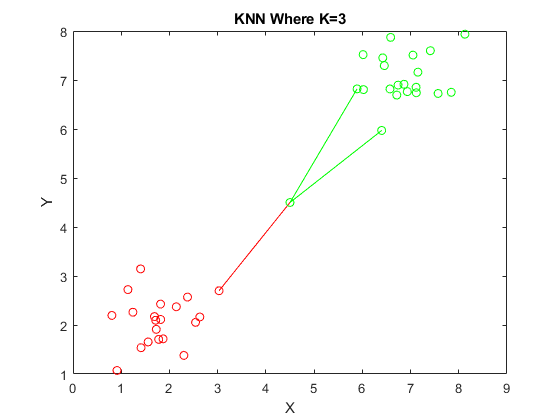
\includegraphics[width=0.5\linewidth, scale=0.5]{Knn3after.png}
	\caption{Looking at the 3 nearest points, the majority classifier is red, so the new point is classified as red.}
\end{figure}

\section{k-Means}

Goal: Find some centers ranging from $\mu_1, \mu_2, ..................,\mu_k$ that minimizes the following equation:
\begin{equation*}  
\sum_{k=1}^{k}\sum_{\rm{x} \in S_k} || \textbf{X}_i-\mu_k||_2^2
\end{equation*}


\begin{equation*} \text{Here } S_k \text{ indicates points that correspond to the }k^{th} \text{ cluster}
\end{equation*}



We will be using \textbf{Lloyd's  Algorithm} to solve the problem of k-Means by using the following steps:

\begin{figure}[H]
	\centering
	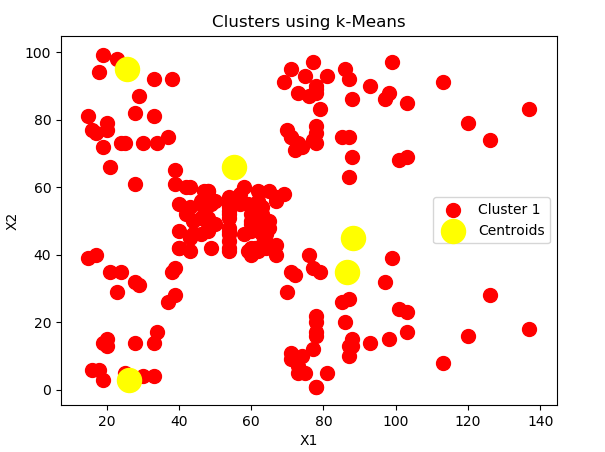
\includegraphics[width=0.5\linewidth, scale=0.5]{initialstep.png}
	\caption{Initial Starting point with all points.}
\end{figure}

\begin{itemize}
  \item Step 0: Initialize $\mu_1, \mu_2, ..................,\mu_k$ 
  \item Step 1: Assign points $\textbf{X}_1, \textbf{X}_2, ..................,\X_N$ to their nearest nearest neighbors center. This will
  produce the sets as $S_1, S_2, ..................,S_N$
  \item Step 2: Compute new centers. The mathematical form is as follows
  \begin{equation*} 
\mu_k =  \frac{1}{|S_k|} \sum_{\rm{x}_i \in S_k} \textbf{X}_i
 \end{equation*}
  
\end{itemize}

 \begin{center}
 Repeat steps 1 and 2 until convergence. We know that the the centers will remain the same when the point of convergence arrives. Refer to figure 8.6 for the final graph.
 \end{center}

  
 \begin{figure}[H]
	\centering
	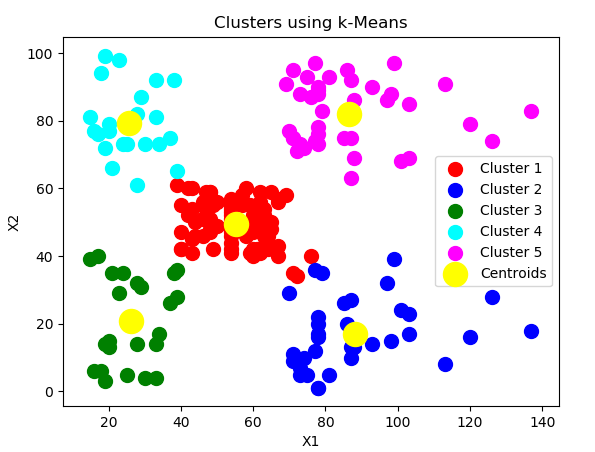
\includegraphics[width=0.5\linewidth, scale=0.5]{finalstep.png}
	\caption{Final graph with total 5 clusters.}
\end{figure}
  
\section{Conclusion}
This lecture shows logic behind Nearest Neighbor, k-Nearest Neighbors and k-Means Clustering.
While Nearest Neighbor and k-Nearest Neighbor predict the class in which a new data point belongs, k-Means classifies an unlabeled data set without any estimate for number of classes into different clusters. Both are completely different methods and they have different applications.

\end{document} 